\documentclass[10pt]{article}

\usepackage{multirow}
\usepackage{rotating,graphicx}
%\usepackage{wrapfig}
\usepackage{amssymb}
\usepackage{amsmath}
\usepackage{lscape}
\usepackage{times}
\usepackage{color}  % For \textcolor and \color % Ex. : \textcolor{red}{Text colored with} ; {\color{red}Text colored with}
\usepackage{soul}   % For \hl{ highlighted text} ; \sethlcolor{colorname}
%\usepackage[table]{xcolor}
\usepackage{xcolor,colortbl}
\usepackage{capt-of}
\usepackage{textcomp}  % allows \textonehalf,  \textonequarter, or else
%\usepackage{mathcomp}  % make it math compatible

\oddsidemargin =-0.6in
\evensidemargin=-0.6in
%\textwidth=7.6in   % owl
 \textwidth=7.8in % laptop
\textheight=10.2in
% \topmargin=-.25in   % owl
 \topmargin=-1.in    % laptop
\footskip=-.0in

\newcommand{\Bl}{\ensuremath{B_{{low}}}}
\newcommand{\Bh}{\ensuremath{B_{{high}}}}
\newcommand{\Il}{\ensuremath{I_{{low}}}}
\newcommand{\Ih}{\ensuremath{I_{{high}}}}
\newcommand{\Br}{\ensuremath{B\! \rho}}
\newcommand{\CE}{concentration ellipse}
\newcommand{\CES}{CE-$\rm \mathcal{S}$}
\newcommand{\dEE}{\small \ensuremath{\frac{dE}{E}}}
\newcommand{\eg}{\ensuremath{\it e.g.}}
\newcommand{\Ha}{\ensuremath{\mathcal{H}}}
\newcommand{\Sa}{\ensuremath{\mathcal{S}}}
\newcommand{\vs}{\ensuremath{\it vs.}}
\newcommand{\ie}{\ensuremath{\it i.e.}}
\newcommand{\hbrk}{\hfill \break}
\newcommand{\sr}{synchrotron radiation}
\newcommand{\SRl}{SR loss}
\newcommand{\x}{\ensuremath{x}} 
\newcommand{\xp}{\ensuremath{{x'}}}
\newcommand{\z}{\ensuremath{z} }
\newcommand{\zp}{\ensuremath{{z'}}}
\newcommand{\y}{\ensuremath{y} }
\newcommand{\yp}{\ensuremath{{y'}}}
\newcommand{\dl}{\ensuremath{{\delta l}}} 
\newcommand{\dE}{\ensuremath{{\delta E}}}
\newcommand{\X}{\ensuremath{X} }
\newcommand{\Xp}{\ensuremath{{X'}}}
\newcommand{\Z}{\ensuremath{Z} }
\newcommand{\zg}{Zgoubi}
\newcommand{\Zp}{\ensuremath{{Z'}}}
\newcommand{\Y}{\ensuremath{Y} }
\newcommand{\Yp}{\ensuremath{{Y'}}}
\newcommand{\Len}{\ensuremath{l} }
\newcommand{\Mom}{\ensuremath{E}}
\newcommand{\Sx}{\ensuremath{\mathcal{S}_x}}
\newcommand{\Sy}{\ensuremath{\mathcal{S}_y}}
\newcommand{\Sz}{\ensuremath{\mathcal{S}_z}}

\newcommand{\C}{\ensuremath{\mathcal{C}}}
\newcommand{\D}{\ensuremath{\mathcal{D}}}
\newcommand{\HH}{\ensuremath{\mathcal{H}}}
\newcommand{\bHH}{\bar \HH}
\newcommand{\com}{{center of mass}}
\newcommand{\lab}{{laboratory frame}}
\newcommand{\LL}{\ensuremath{\mathcal{L}}}
\newcommand{\rms}{\ensuremath{rms}}
\newcommand{\wrt}{{with respect to}}

\newcommand{\bull}{\ensuremath{\bullet~}}
\newcommand{\cf}{\ensuremath{\textsl{cf.}}}
\newcommand{\bhel}{\ensuremath{\mathbf{^3He^{2+}}}}
\newcommand{\hel}{\ensuremath{\mathrm{^3He^{2+}}}}
\newcommand{\nib}{\noindent \ensuremath{\bullet~}}
\newcommand{\snib}{\noindent {\small \ensuremath{\bullet~}}}
\newcommand{\nid}{\noindent \ensuremath{\diamond~}}
\newcommand{\snid}{\noindent {\small \ensuremath{\diamond~}}}
\newcommand{\nin}{\noindent~}
\newcommand{\no}{\ensuremath{\mathbf{\vec n_0}}}
\newcommand{\MC}{Monte~Carlo}
\newcommand{\p}{\ensuremath{\mathbf{p}}}
\newcommand{\pp}{$\rm p\! \! \uparrow$}

\definecolor{orange}{rgb}{1,0.5,0}
\definecolor{yelloworange}{rgb}{1,.647,0}
\newcommand{\black}{\color{black}}
\newcommand{\red}{\color{red}}
\newcommand{\green}{\color{green}}
\newcommand{\blue}{\color{blue}}
\newcommand{\yo}{\color{yelloworange}}

\newcommand{\referenceA}{\rm  }
\newcommand{\referenceB}{\rm }
\newcommand{\referenceC}{\rm }

\pagestyle{headings}
\markboth{\small  \referenceA ~ ~   \referenceB ~ ~  \referenceC \hfill }
         {\small  \referenceA ~ ~   \referenceB ~ ~  \referenceC \hfill }


\begin{document}

\thispagestyle{empty}

\begin{minipage}{1.\linewidth}
\bf
  \flushright{F. M\'eot}
\vspace{-2ex}
  
  \flushright{BNL C-AD}
\vspace{-2ex}
  
  \flushright{Zgoubi 2019 Workshop, Boulder, CO}
\vspace{-2ex}
  
\flushright{24-29 Aug. 2019} 
\end{minipage}


\vspace{5ex}

\centerline{\LARGE \bf
 A Second Order Quadrupole Doublet Achromat
}


\vspace{5ex}
\author{
F.~M\'eot
\\
Collider-Accelerator Department, BNL, Upton, NY 11973 \\
}



EBMULT is used in this exercise (pp.~129 and 224 in the Users' Guide).  $ \vec B$ and $ \vec E$ are set so to ensure
focal distance as desired, and cancelation of the second order chromatic aberrations inherent to electromagnetic quadrupoles.

REBELOTE is used to track 100,000s of particles, for statistics purposes, and FAISTORE to log them to zgoubi.fai.
IMAGE is used ot locate the beam waist, HISTO is used to get transverse beam densities. 


\section*{Working hypotheses}

\nib The pair of E$\times$B quadrupoles is sketched in the figure below. The probe is assumed to be a 20\,keV proton beam.

~

\mbox{
\begin{minipage}{0.4\linewidth}
\hspace{-10mm}
  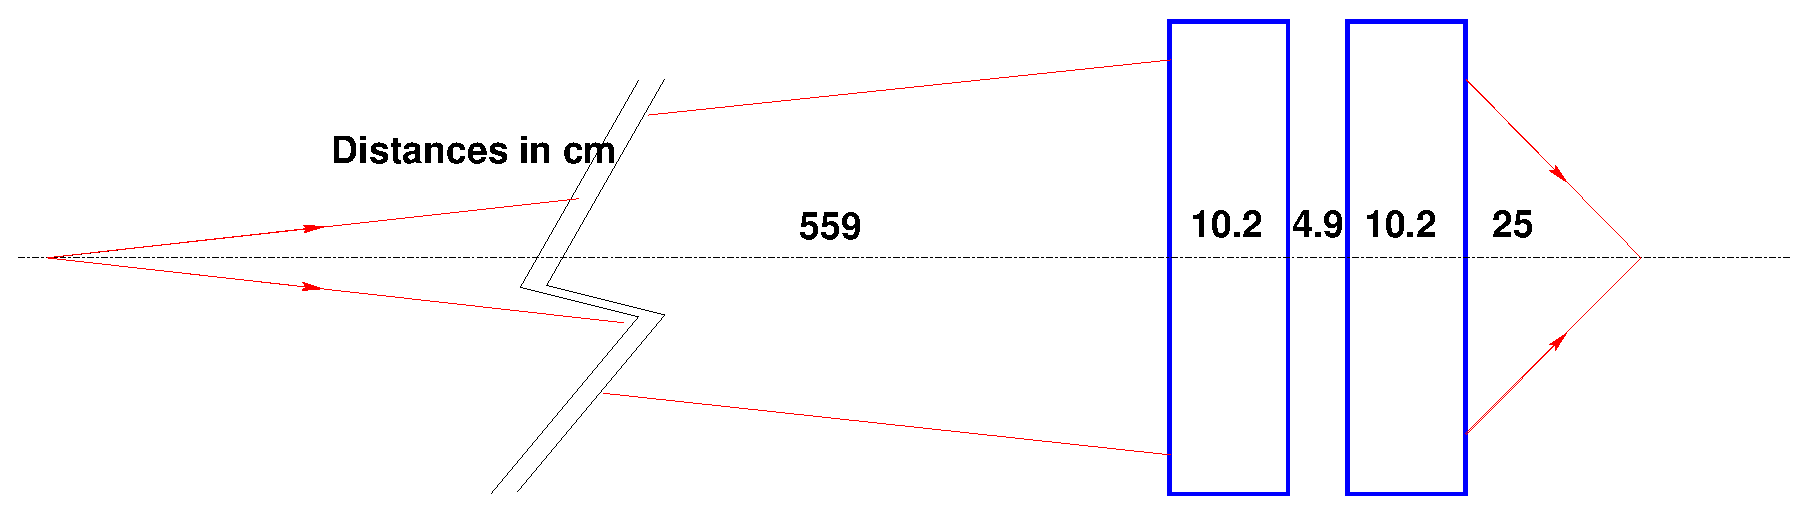
\includegraphics[width=1.3\linewidth]{achromat.eps}
\end{minipage} \hfill
\begin{minipage}{0.3\linewidth}
\centering
$\left\{ \begin{array}{l} E_Y = -KY = -\partial V_{El} /\partial Y \\ E_Y = +KZ = -\partial V_{El} /\partial Z \end{array} \right. $ 


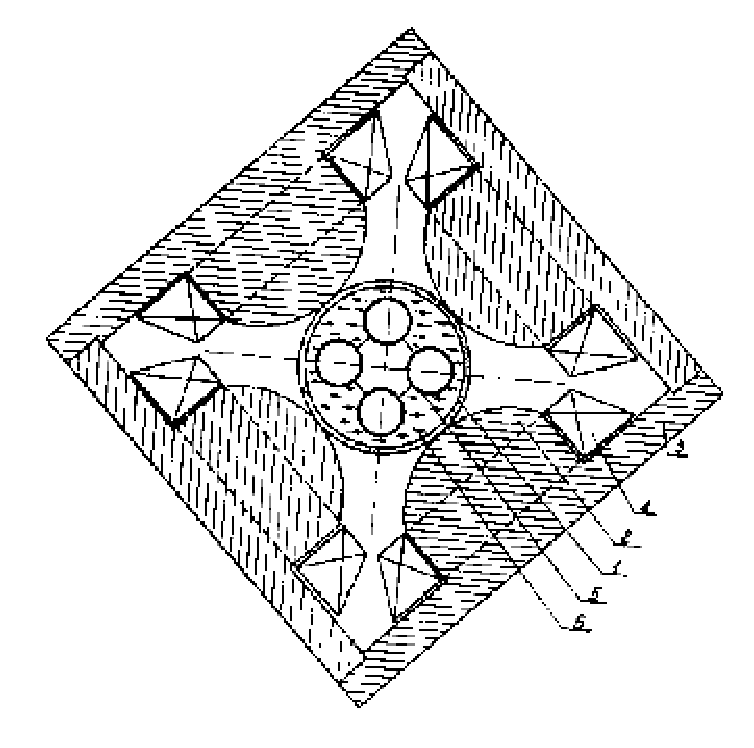
\includegraphics[width=0.55\linewidth]{EBQuad.eps}

  Ref.: S.Ya.~Yavor, NIM A 26 (1964)
\end{minipage}
\begin{minipage}{0.3\linewidth}
\centering
thus, in the upright frame:  $V_{El} = \dfrac{K}{2}(Y^2-Z^2)$

~

In the rotated frame: $\left[ \begin{array}{c} U \\ V \end{array}\right]  = \left[ \begin{array}{cc} \cos 45^o & -\sin45^o \\ V\sin45^o & \cos45^o\end{array} \right] \left[ \begin{array}{c} Y \\ Z \end{array}\right]$

~

 equipotentials: $V_{El} = K UV$.

Thus, the 45$^o$ rotated equipotentials of an electrostatic quad realize the same focusing effect as a magnetic quadrupole.

\end{minipage}
}

\section*{ Numerical experience }

\nin 1/ Let's  walk through the fortran, see what happens when the execution pointer meets 'EBMULT' in zgoubi.dat sequence...

Open zgoubi.f $\Rightarrow$ look for EBMULT. Look into include/LSTKEY.H  $\Rightarrow$  look for 'CALL REBMULT', look into rebmul.f
$\Rightarrow$  look for 'CALL QUASEX', look into quasex.f $\Rightarrow$ look for 'CALL CHXC', look into chxc.f, look for
EBMULT therein (you won't find it, figure out why)
$\Rightarrow$ look for 'CALL TRANSF' in quasex, look into transf.f $\Rightarrow$ look into integr.f: it pushes the particles, one by one,
through EBMULT (and any other element) $\Rightarrow$  look for 'CALL CHAMC', 'CALL CHAMK', 'CALL DEVTRA'.

~

\nin 2/ Install in Zgoubi the optical sequence above, leaving first the electric component zero, with B
such as to provide the proper image distance.

Produce the transport matrices to 3rd order. 

~

\nin 3/ Switch on the E component, setting both E and B to preserve the image distance.

Produce the transport matrices to 3rd order, compare with the previous case.

~

\nin 4/ Using REBELOTE, track 100,000 particles through the achromat. Use IMAGE to localize the waist.

set the final straight to the waist distance,  use HISTO to provide Y and Z transverse beam densities at the image.


\end{document}
